% !TeX program = PdfLaTeX
% !TeX root = ../../Elaborati_Aerodinamica_Bruno_Spoti.tex
\chapter{Effetti viscosi}

In questo capitolo sarà studiata l’aerodinamica del profilo alare  PW106 ad assetti piccoli e medi, tenendo conto degli effetti viscosi. \\ A tal proposito in primo luogo saranno esaminati gli effetti della variazione del numero di Reynolds sulle curve di portanza e sulla polare, analizzandone alcuni casi più significativi, al fine di evidenziare l’effetto che ha la variazione di tale valore adimensionale sulle prestazioni del profilo. Verrà, inoltre, analizzata la variazione del coefficiente di pressione dovuta agli effetti di scala. Saranno, poi, presi in considerazione i più significativi parametri di strato limite e saranno analizzati gli effetti della transizione forzata, fissata ad un certo valore della corda, e quelli che il parametro $n_{cr}$, che tiene conto degli effetti di turbolenza e rugosità, sull’aerodinamica del profilo.\\
Tali analisi saranno condotte mediante l’ausilio di XFOIL. 

\section{Curva di Portanza e polare}

Il profilo analizzato è un profilo progettato per lavorare a bassi numeri di Reynolds. Nella curva di Portanza ottenuta con XFOIL, tuttavia, anche a $Re$ più elevati, non si riscontrano particolari oscillazioni, pertanto sono stati scelti i seguenti valori: \\

\begin {itemize}
\item $Re=5\times10^5  $ ${\to}$ $ {\alpha}_\mathrm{stall}=13^\circ$  ${\to}$ $C_{l_\mathrm{max}}=1.28$;
\item $Re=1\times10^6$ ${\to}$ $ {\alpha}_\mathrm{stall}=13^\circ$  ${\to}$ $C_{l_\mathrm{max}}=1.38$;
\item $Re=3\times10^6$ ${\to}$ $ {\alpha}_\mathrm{stall}=16^\circ$  ${\to}$ $C_{l_\mathrm{max}}=1.56$;
\item $Re=1\times10^7$ ${\to}$ $ {\alpha}_\mathrm{stall}=18^\circ$  ${\to}$ $C_{l_\mathrm{max}}=1.76$.
\end{itemize}

\noindent \\
Dall'osservazione dei grafici riportati nelle figure \ref{fig:cla11} e \ref{fig:pol} si notano alcuni degli effetti che ha l’incremento del numero di Reynolds sulle prestazioni del profilo. Al crescere di $Re$, la curva di portanza aumenta il suo tratto lineare, il che vuol dire che aumenta il $C_{l_\mathrm{max}}$ e, conseguentemente, l’angolo di stallo. Dalle polari del profilo si nota la progressiva diminuzione del $C_{d_\mathrm{min}}$ al crescere del numero di Reynolds connesso al già citato aumento del $C_{l_\mathrm{max}}$.

\begin{figure} [H]
\centering
\begin{tikzpicture} 
\begin{axis} [ 
legend style={at={(0.3,0.98)}},
ylabel style={rotate=-90}, xmin=-20, 
xmax=25, 
ymin=-2,
ymax=2,
xlabel=${\alpha}$,
ylabel=$C_l$ ,
width=12cm,
height=19 cm,
scale only axis,
grid=major] 
\addplot [black, smooth,mark=*]
file{images/fileDat/EffettiViscosi/Cl_vs_alpha_Re_5_10_5.dat};
\addplot [black,smooth,mark=square]
file{images/fileDat/EffettiViscosi/Cl_vs_alpha_Re_1_10_6.dat};
\addplot [black, smooth,mark=diamond*]
file{images/fileDat/EffettiViscosi/Cl_vs_alpha_Re_3_10_6.dat};
\addplot [black, smooth,mark=star]
file{images/fileDat/EffettiViscosi/Cl_vs_alpha_Re_1_10_7.dat};
\legend {$Re=5\times10^5  $,$Re=1\times10^6$,$Re=3\times10^6$,$Re=1\times10^7$}
\end{axis}
\end{tikzpicture} 
\caption{\footnotesize Profilo alare PW106, confronto delle curve di portanza al variare del numero di Reynolds. XFOIL 6.99 }
\label{fig:cla11}
\end{figure}

\begin{figure} [H]
\centering
\begin{tikzpicture} 
\begin{axis} [ 
legend style={at={(0.98,0.30)}},
ylabel style={rotate=-90}, xmin=0, 
ymin=-2,
ymax=2.2,
xlabel=$C_d$ (drag count),
ylabel=$C_l$ ,
width=11cm,
height=11cm,
scale only axis,
grid=major] 
\addplot [black, smooth,mark=*]
file{images/fileDat/EffettiViscosi/cd_cl_5_10_5.dat};
\addplot [black,smooth,mark=square]
file{images/fileDat/EffettiViscosi/cd_cl_10_6.dat};
\addplot [black, smooth,mark=diamond*]
file{images/fileDat/EffettiViscosi/cd_cl_3_10_6.dat};
\addplot [black, smooth,mark=star]
file{images/fileDat/EffettiViscosi/cd_cl_10_7.dat};
\legend {$Re=5\times10^5  $,$Re=1\times10^6$,$Re=3\times10^6$,$Re=1\times10^7$}
\end{axis}
\end{tikzpicture}
\caption{\footnotesize Profilo alare PW106, confronto delle polari al variare del numero di Reynolds. XFOIL 6.99 }
\label{fig:pol}
\end{figure}

\begin{figure} [H]
\centering
\begin{tikzpicture} 
\begin{axis} [ 
legend style={at={(0.98,0.90)}},
ylabel style={rotate=-90}, xmin=0, 
xmax=250, 
ymin=-1,
ymax=1,
xlabel=$C_d$ (drag count),
ylabel=$C_l$ ,
width=9cm,
height=6cm,
scale only axis,
grid=major] 
\addplot [black, smooth,mark=*]
file{images/fileDat/EffettiViscosi/cd_cl_5_10_5.dat};
\addplot [black,smooth,mark=square]
file{images/fileDat/EffettiViscosi/cd_cl_10_6.dat};
\addplot [black, smooth,mark=diamond*]
file{images/fileDat/EffettiViscosi/cd_cl_3_10_6.dat};
\addplot [black, smooth,mark=star]
file{images/fileDat/EffettiViscosi/cd_cl_10_7.dat};
\legend {$Re=5\times10^5 $,$Re=1\times10^6$,$Re=3\times10^6$,$Re=1\times10^7$}
\end{axis}
\end{tikzpicture}
\caption{\footnotesize Polari del profilo PW106 al variare del numero di Reynolds, zoom della zona di alta e media velocità. XFOIL 6.99 }
\label{fig:pol}
\end{figure}


\section{Coefficiente di pressione al variare del numero di Reynolds }

\noindent \\ 

Di seguito sono confrontati i grafici del $C_p$ ad un certo angolo d’attacco del profilo e fissato $n_{cr}$, per vari numeri di Reynolds così da vedere la formazione e l’evoluzione delle bolle laminari in dipendenza dal Re. Successivamente si vedrà l’effetto della variazione di ${\alpha}$  ad un fissato numero di Reynolds. \\
Gli sviluppi applicativi, in questo capitolo, saranno fatti in condizioni di piccoli e medi angoli d'attacco, rimandando al successivo capitolo lo studio dell'alta portanza.\\
Preliminarmente, al fine di comprendere le differenze tra la soluzione Euleriana e quella viscosa, sarà graficato l'andamento del $C_p$ per il profilo PW106 ad un fissato angolo d’attacco, in assenza di effetti viscosi, e con un $Re=2.5\times10^5$.\\


\begin{figure} [H]
\centering
\begin{tikzpicture} 
\begin{axis} [ 
ylabel style={rotate=-90}, xmin=0, 
xmax=1, 
ymin=-2,
ymax=1,
xlabel=$\frac{x}{c}$, 
ylabel=$C_p$ ,
 y dir=reverse,
width=12cm,
height=6 cm,
scale only axis,
grid=major] 
\addplot [black,thin]
file{images/fileDat/EffettiViscosi/Cp_alfa_3_Invdorso.dat};
\addplot [black,thin,dashed]
file{images/fileDat/EffettiViscosi/Cp_alfa_3_Invventre.dat};
\addplot [black,ultra thick]
file{images/fileDat/EffettiViscosi/Cp_alfa_3_Re_2.5_10e5dorso.dat};
\addplot [black,ultra thick,dashed]
file{images/fileDat/EffettiViscosi/Cp_alfa_3_Re_2.5_10e5ventre.dat};
\draw[rotate=-2] (0.44, -0.5) ellipse (0.15 and 0.3);
\legend {Soluzione Euleriana dorso, Soluzione Euleriana ventre, Soluzione viscosa  dorso $Re=2.5\times10^5$, Soluzione viscosa ventre $Re=2.5\times10^5$}
\end{axis}
\end{tikzpicture}
\caption{\footnotesize Profilo PW106, confronto del coefficiente di pressione $ \alpha=3^\circ$. Soluzione Euleriana ed effetti viscosi. XFOIL 6.99}\label{fig:cpre}
\end{figure}
\noindent  \\

Dalla figura \ref{fig:cpre} si nota una sostanziale differenza tra la distribuzione del $C_p$ Euleriano e quello ottenuto considerando gli effetti della viscosità. In quest'ultimo si nota un {\itshape plateau} di pressione, ossia una zona ove il $C_p$ non aumenta né diminuisce. Questo fenomeno è dovuto alla presenza di una {\itshape bolla laminare}, cioè una zona ove il flusso separa laminare e riattacca turbolento. La bolla laminare individua una parte del campo (sotto) ove il flusso è reverso e una (sopra) ove il flusso è diretto. Il fenomeno della bolla laminare si presenta in maniera più evidente a bassi numeri di Reynolds, pertanto per le successive applicazioni lavoreremo a $Re$ non elevati.

\begin{figure} [H]
\centering
\begin{tikzpicture} 
\begin{axis} [ 
ylabel style={rotate=-90}, xmin=0, 
xmax=1, 
ymin=-1,
ymax=1,
xlabel=$\frac{x}{c}$, 
ylabel=$C_p$ ,
 y dir=reverse,
width=12cm,
height=7 cm,
scale only axis,
grid=major] 
\addplot [black,very thin]
file{images/fileDat/EffettiViscosi/Cp_alfa_0_Re_2.5_10e5dorso.dat};
\addplot [black,semithick]
file{images/fileDat/EffettiViscosi/Cp_alfa_0_Re_5_10e5dorso.dat};
\addplot [black,ultra thick]
file{images/fileDat/EffettiViscosi/Cp_alfa_0_Re_1_10e6dorso.dat};
\addplot [black,very thin, dashed]
file{images/fileDat/EffettiViscosi/Cp_alfa_0_Re_2.5_10e5ventre.dat};
\addplot [black,semithick, dashed]
file{images/fileDat/EffettiViscosi/Cp_alfa_0_Re_5_10e5ventre.dat};
\addplot [black,ultra thick, dashed]
file{images/fileDat/EffettiViscosi/Cp_alfa_0_Re_1_10e6ventre.dat};
\draw[rotate=-2] (0.6, -0.2) ellipse (0.15 and 0.3);
\legend {$Re=2.5\times10^5$,$Re=5\times10^5  $,$Re=1\times10^6$}
\end{axis}
\end{tikzpicture}
\caption{\footnotesize Profilo alare PW106, confronto del coefficiente di pressione $ \alpha=0^\circ$ sul dorso del profilo (linea continua) e sul ventre (linea tratteggiata) al variare del numero di Reynolds. XFOIL 6.99}\label{fig:cpre1}
\end{figure}
\noindent \\ \\ 

\begin{figure} [H]
\centering
\begin{tikzpicture} 
\begin{axis} [ 
ylabel style={rotate=-90}, xmin=0, 
xmax=1, 
ymin=-1,
ymax=1,
xlabel=$\frac{x}{c}$, 
ylabel=$C_p$ ,
 y dir=reverse,
width=12cm,
height=7 cm,
scale only axis,
grid=major] 
\addplot [black,very thin]
file{images/fileDat/EffettiViscosi/Cp_alfa_2_Re_2.5_10e5dorso.dat};
\addplot [black,semithick]
file{images/fileDat/EffettiViscosi/Cp_alfa_2_Re_5_10e5dorso.dat};
\addplot [black,ultra thick]
file{images/fileDat/EffettiViscosi/Cp_alfa_2_Re_1_10e6dorso.dat};
\addplot [black,very thin, dashed]
file{images/fileDat/EffettiViscosi/Cp_alfa_2_Re_2.5_10e5ventre.dat};
\addplot [black,semithick, dashed]
file{images/fileDat/EffettiViscosi/Cp_alfa_2_Re_5_10e5ventre.dat};
\addplot [black,ultra thick, dashed]
file{images/fileDat/EffettiViscosi/Cp_alfa_2_Re_1_10e6ventre.dat};
\draw[rotate=-7] (0.51, -0.54) ellipse (0.15 and 0.23);
\legend {$Re=2.5\times10^5$,$Re=5\times10^5  $,$Re=1\times10^6$,$Re=2.5\times10^5$}
\end{axis}
\end{tikzpicture}
\caption{\footnotesize Profilo alare PW106, confronto del coefficiente di pressione $ \alpha=2^\circ$ sul dorso del profilo (linea continua) e sul ventre (linea tratteggiata) al variare del numero di Reynolds. XFOIL 6.99}\label{fig:cpre2}
\end{figure}
\noindent 

\begin{figure} [H]
\centering
\begin{tikzpicture} 
\begin{axis} [ 
ylabel style={rotate=-90}, xmin=0, 
xmax=1, 
ymin=-1.5,
ymax=1,
xlabel=$\frac{x}{c}$, 
ylabel=$C_p$ ,
 y dir=reverse,
width=12cm,
height=7 cm,
scale only axis,
grid=major] 
\addplot [black,very thin]
file{images/fileDat/EffettiViscosi/Cp_alfa_4_Re_2.5_10e5dorso.dat};
\addplot [black,semithick]
file{images/fileDat/EffettiViscosi/Cp_alfa_4_Re_5_10e5dorso.dat};
\addplot [black,ultra thick]
file{images/fileDat/EffettiViscosi/Cp_alfa_4_Re_1_10e6dorso.dat};
\addplot [black,very thin, dashed]
file{images/fileDat/EffettiViscosi/Cp_alfa_4_Re_2.5_10e5ventre.dat};
\addplot [black,semithick, dashed]
file{images/fileDat/EffettiViscosi/Cp_alfa_4_Re_5_10e5ventre.dat};
\addplot [black,ultra thick, dashed]
file{images/fileDat/EffettiViscosi/Cp_alfa_4_Re_1_10e6ventre.dat};
\draw[rotate=-9] (0.38, -0.8) ellipse (0.15 and 0.3);
\legend {,$Re=2.5\times10^5$,$Re=5\times10^5  $,$Re=1\times10^6$}
\end{axis}
\end{tikzpicture}
\caption{\footnotesize Profilo alare PW106, confronto del coefficiente di pressione $ \alpha=4^\circ$  sul dorso del profilo (linea continua) e sul ventre (linea tratteggiata) al variare del numero di Reynolds. XFOIL 6.99}\label{fig:cpre3}
\end{figure}
\noindent 


Man mano che diminuisce il numero di Reynolds la bolla si allunga e si sposta verso il bordo d'uscita, mentre all'aumentare dell'angolo di attacco, la bolla si sposta verso il LE.\\ Per vedere ciò al variare di $\alpha$ si guardi il seguente grafico, fatto per un numero di Reynolds non troppo alto per visualizzare meglio la presenza delle bolle.

\begin{figure} [H]
\centering
\begin{tikzpicture} 
\begin{axis} [ 
ylabel style={rotate=-90}, xmin=0, 
xmax=1, 
ymin=-1.5,
ymax=1,
xlabel=$\frac{x}{c}$, 
ylabel=$C_p$ ,
 y dir=reverse,
width=12cm,
height=7 cm,
scale only axis,
grid=major] 
\addplot [black,very thin]
file{images/fileDat/EffettiViscosi/Cp_alfa_0_Re_2.5_10e5dorso.dat};
\addplot [black,semithick]
file{images/fileDat/EffettiViscosi/Cp_alfa_2_Re_2.5_10e5dorso.dat};
\addplot [black,ultra thick]
file{images/fileDat/EffettiViscosi/Cp_alfa_4_Re_2.5_10e5dorso.dat};
\addplot [black,very thin, dashed]
file{images/fileDat/EffettiViscosi/Cp_alfa_0_Re_2.5_10e5ventre.dat};
\addplot [black,semithick, dashed]
file{images/fileDat/EffettiViscosi/Cp_alfa_2_Re_2.5_10e5ventre.dat};
\addplot [black,ultra thick, dashed]
file{images/fileDat/EffettiViscosi/Cp_alfa_4_Re_2.5_10e5ventre.dat};
\legend {$\alpha=0^\circ $,$\alpha = 2^\circ$,$ \alpha=4^\circ$}
\end{axis}
\end{tikzpicture}
\caption{\footnotesize Profilo PW106, confronto del Coefficiente di Pressione al variare dell'angolo d'attacco sul dorso del profilo (linea continua) e sul ventre (linea tratteggiata), $Re= 2.5\times10^5$. XFOIL 6.99}\label{fig:cpre4}
\end{figure}
\noindent 

\section{Sviluppo e parametri di Strato Limite}

\noindent \\


Gli effetti viscosi dell'aerodinamica applicata possono essere ritenuti confinati all'interno di una sottile zona in prossimità del corpo, detta \emph{strato limite}, pertanto è sicuramente interessante vedere come cambia lo sviluppo dello strato limite all'aumentare dell'angolo d'attacco e come variano i parametri di strato limite al variare del numero di Reynolds e dell'angolo d'attacco, limitandoci sempre all'analisi di piccoli e medi assetti.\\
\begin{figure}[H]
\centering
\subfloat[][$\alpha=0^\circ$]
{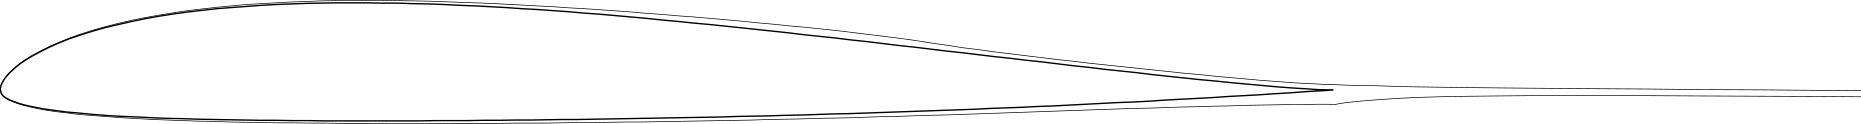
\includegraphics[width=.95\textwidth]{images/fileImg/alfa0_Re_25e4.png}} \\
\subfloat[][$\alpha=2^\circ$]
{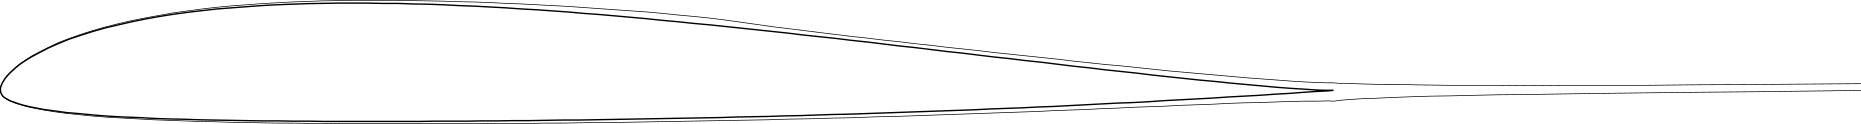
\includegraphics[width=.95\textwidth]{images/fileImg/alfa2_Re_25e4.png}} \\
\subfloat[][$\alpha=4^\circ$]
{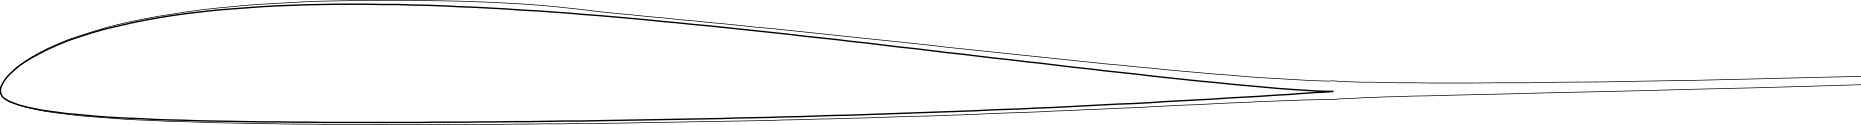
\includegraphics[width=.95\textwidth]{images/fileImg/alfa4_Re_25e4.png}} 
\caption{\footnotesize Profilo PW106, sviluppo dello strato limite, $Re=2.5\times10^5$, $n_{cr}$=9, transizione libera. XFOIL 6.99}
\label{fig:subfig}
\end{figure}


\noindent \\

Dalla figura~\vref{fig:subfig} si puó notare il lieve "rigonfiamento" dello strato limite in corrispondenza della bolla laminare che si sposta verso il bordo d'attacco all'aumentare di ${\alpha}$.\\ \\
Per studiare la dinamica delle bolle laminari, è necessario far riferimento all'evoluzione dei parametri di strato limite lungo il profilo. La presenza di una bolla, difatti, é accompagnata da una forte crescita del fattore di forma H come si vede in figura~\vref{fig:acca} e da un intervallo di valori negativo per quanto riguarda il coefficiente di attrito   $C_f$. La presenza delle bolle laminari è evidenziata da figura~\vref{fig:acca} a  figura~\vref{fig:fig4.13} mediante un'ellisse.

\begin{figure} [H]
\centering
\begin{tikzpicture} 
\begin{axis} [ 
legend style={at={(0.9,0.98)}},
ylabel style={rotate=-90}, xmin=0, 
xmax=2.02, 
ymin=0,
ymax=5,
xlabel=$\frac{s}{c}$, 
ylabel=$H$ ,
width=12cm,
height=7 cm,
scale only axis,
grid=major] 
\addplot [black,very thin,smooth]
file{images/fileDat/EffettiViscosi/H_alfa0_Re_25e4.dat};
\addplot [black,semithick, smooth]
file{images/fileDat/EffettiViscosi/H_alfa0_Re_5e5.dat};
\addplot [black,ultra thick,smooth]
file{images/fileDat/EffettiViscosi/H_alfa0_Re_1e6.dat};
\draw (0.4, 3) ellipse (0.2 and 1.9);
\legend {$Re=2.5\times10^5$,$Re=5\times10^5  $,$Re=1\times10^6$}
\end{axis}
\end{tikzpicture}
\caption{\footnotesize Profilo alare PW106, confronto dell'andamento del fattore di forma H al variare del numero di Reynolds, $\alpha=0^\circ$. XFOIL 6.99}\label{fig:acca}
\end{figure}
\noindent \\ \\ 



\begin{figure} [H]
\centering
\begin{tikzpicture} 
\begin{axis} [ 
ylabel style={rotate=-90}, xmin=0, 
xmax=2.02, 
ymin=-0.01,
ymax=0.04,
xlabel=$\frac{s}{c}$, 
ylabel=$C_f$ ,
width=12cm,
height=7 cm,
scale only axis,
grid=major] 
\addplot [black,very thin,smooth]
file{images/fileDat/EffettiViscosi/Cf_alfa0_Re_25e4.dat};
\addplot [black,semithick, smooth]
file{images/fileDat/EffettiViscosi/Cf_alfa0_Re_5e5.dat};
\addplot [black,ultra thick,smooth]
file{images/fileDat/EffettiViscosi/Cf_alfa0_Re_1e6.dat};
\draw (0.38, 0.002) ellipse (0.2 and 0.01);
\legend {$Re=2.5\times10^5$,$Re=5\times10^5  $,$Re=1\times10^6$}
\end{axis}
\end{tikzpicture}
\caption{\footnotesize Profilo alare PW106, confronto dell'andamento del coefficiente d'attrito $C_f$ al variare del numero di Reynolds, $\alpha=0^\circ$. XFOIL 6.99}\label{fig:cie}
\end{figure}
\noindent \\ \\ 

Dai grafici \ref{fig:acca} e \ref{fig:cie} si vede che a circa l' 60\% della corda, sul dorso del profilo, c'é una bolla laminare individuata da un intervallo di valori per i quali il $C_f$ è negativo per $Re=2.5 \times 10^5$ e $Re=5 \times 10^5$, ció non accade a numeri di Reynolds piú elevati.

È interessante, inoltre, vedere come variano i parametri di strato limite fissato il $Re$, a vari angoli d'attacco (figura~\vref{fig:fig4.12} e~\vref{fig:fig4.13}).

\begin{figure} [H]
\centering
\begin{tikzpicture} 
\begin{axis} [ 
ylabel style={rotate=-90}, xmin=0, 
xmax=2.02, 
ymin=0,
ymax=6.5,
xlabel=$\frac{s}{c}$,
ylabel=$H$ ,
width=12cm,
height=6.4 cm,
scale only axis,
grid=major] 
\addplot [black,very thin,smooth]
file{images/fileDat/EffettiViscosi/H_alfa0_Re_25e4.dat};
\addplot [black,semithick, smooth]
file{images/fileDat/EffettiViscosi/H_alfa2_Re_25e4.dat};
\addplot [black,ultra thick,smooth]
file{images/fileDat/EffettiViscosi/H_alfa4_Re_25e4.dat};
\draw (0.5, 3.1) ellipse (0.36 and 2.2);
\legend {$\alpha=0 $,$\alpha = 2$,$ \alpha=4$}
\end{axis}
\end{tikzpicture}
\caption{\footnotesize Profilo alare PW106, confronto dell'andamento del fattore di forma H al variare dell'angolo d'attacco, $Re=2.5\times10^5$. XFOIL 6.99 }
\label{fig:fig4.12}
\end{figure}
\noindent 

\begin{figure} [H]
\centering
\begin{tikzpicture} 
\begin{axis} [ 
ylabel style={rotate=-90}, xmin=0, 
xmax=2.02, 
ymin=-0.01,
ymax=0.07,
xlabel=$\frac{s}{c}$, 
ylabel=$C_f$ ,
width=12cm,
height=6.4 cm,
scale only axis,
grid=major] 
\addplot [black,very thin,smooth]
file{images/fileDat/EffettiViscosi/Cf_alfa0_Re_25e4.dat};
\addplot [black,semithick, smooth]
file{images/fileDat/EffettiViscosi/Cf_alfa2_Re_25e4.dat};
\addplot [black,ultra thick,smooth]
file{images/fileDat/EffettiViscosi/Cf_alfa4_Re_25e4.dat};
\draw (0.53, 0.002) ellipse (0.26 and 0.01);
\legend {$\alpha=0 $,$\alpha = 2$,$ \alpha=4$}
\end{axis}
\end{tikzpicture}
\caption{\footnotesize Profilo alare PW106, confronto dell'andamento del coefficiente d'attrito $C_f$ al variare dell'angolo d'attacco, $Re=2.5\times10^5$. XFOIL 6.99}
\label{fig:fig4.13}
\end{figure}
\noindent 

\section{Effetto della Transizione Forzata}
Forzare la transizione vuol dire anticipare il punto ove il flusso intorno al profilo diventa turbolento e, quindi, energizzarlo.\\
Se la transizione viene fissata prima della separazione, e, quindi, di un’eventuale bolla laminare, il flusso divenuto turbolento non separa più da laminare, determinando la scomparsa della bolla stessa.
Di seguito si esamineranno gli effetti della transizione forzata sul grafico del $C_p$ e sui grafici che descrivono i parametri di strato limite più significativi in tal senso: H e $C_f$.\\
Al fine di illustrare la scomparsa della bolla laminare a seguito di una transizione forzata che anticipa la separazione, si condurrà l’analisi a $Re=2.5\times10^5$ valore per il quale si è vista la presenza di una bolla laminare.

Sono stati assunti i seguenti valori:
\begin {itemize}
\item $Re=2.5\times10^5  $ ;
\item $ \alpha=2^\circ$.
\item $n_{cr}=9$
\end{itemize}
La transizione libera, calcolata con XFOIL, avviene (sul dorso) al seguente valore dell'ascissa adimensionalizzata con la corda: 
\begin{equation}
\frac{x_\mathrm{free-transit}}{c}= 0.539
\end {equation}
\noindent
È stata forzata la transizione sul dorso ad un valore di ${\frac{x}{c}}=0.300$ .\\
Di seguito sono riportati graficamente gli effetti che ne derivano.
\begin{figure} [H]
\centering
\begin{tikzpicture} 
\begin{axis} [ 
legend style={at={(0.98,0.98)}},
ylabel style={rotate=-90}, xmin=0, 
xmax=1, 
ymin=-1,
ymax=1,
xlabel=$\frac{x}{c}$, 
ylabel=$C_p$ ,
 y dir=reverse,
width=12cm,
height=7 cm,
scale only axis,
grid=major] 
\addplot [black,very thin]
file{images/fileDat/EffettiViscosi/Cp_alfa_2_Re_2.5_10e5dorso.dat};
\addplot [black, very thick]
file{images/fileDat/EffettiViscosi/Cp_alpha2_Re25e4_xtr0.3dorso.dat};
\addplot [black,very thin, dashed]
file{images/fileDat/EffettiViscosi/Cp_alfa_2_Re_2.5_10e5ventre.dat};
\addplot [black, very thick, dashed]
file{images/fileDat/EffettiViscosi/Cp_alpha2_Re25e4_xtr0.3ventre.dat};
\legend {$Transizione \ libera \ ( 53.9\%)$ , $Transizione \ forzata \ (30\%) $}
\end{axis}
\end{tikzpicture}
\caption{\footnotesize Profilo alare PW106, confronto del coefficiente di pressione sul dorso del profilo (linea continua) e sul ventre (linea tratteggiata) a diversi valori del punto di Transizione sul dorso.  $ \alpha=2^\circ$ , $ Re= 2.5\times10^5$. XFOIL 6.99}\label{fig:caso}
\end{figure}
\noindent

Dalle figure \ref{fig:nona} e \ref{fig:decima} si vede come anticipando la transizione il picco del fattore di forma dello strato limite H scompare e $C_f$ non assume valori negativi. Ciò conferma che non vi è più una bolla laminare sul dorso del profilo in quanto la transizione avviene prima della separazione.
\begin{figure} [H]
\centering
\begin{tikzpicture} 
\begin{axis} [ 
ylabel style={rotate=-90}, xmin=0, 
xmax=2.02, 
ymin=1,
ymax=6,
xlabel=$\frac{s}{c}$,
ylabel=$H$ ,
width=12cm,
height=7cm,
scale only axis,
grid=major] 
\addplot [black,very thin,smooth]
file{images/fileDat/EffettiViscosi/H_alfa2_Re_25e4.dat};
\addplot [black,very thick, smooth]
file{images/fileDat/EffettiViscosi/H_alfa2_Re_25e4_xtr0.3.dat};
\legend {$Transizione \ libera \ ( 53.9\%)$ , $Transizione \ forzata \ (30\%) $}
\end{axis}
\end{tikzpicture}
\caption{\footnotesize Profilo PW106, confronto dell'andamento del fattore di forma H al variare del punto di Transizione sul dorso.  $ \alpha=2^\circ$ , $ Re= 2.5\times10^5$. XFOIL 6.99}\label{fig:decima}
\end{figure} 

\begin{figure} [H]
\centering
\begin{tikzpicture} 
\begin{axis} [ 
legend style={at={(0.98,0.98)}},
ylabel style={rotate=-90}, xmin=0, 
xmax=2.02, 
ymin=-0.01,
ymax=0.05,
xlabel=$\frac{s}{c}$,
ylabel=$C_f$ ,
width=12cm,
height=7.5cm,
scale only axis,
grid=major] 
\addplot [black,very thin,smooth]
file{images/fileDat/EffettiViscosi/Cf_alfa2_Re_25e4.dat};
\addplot [black,very thick, smooth]
file{images/fileDat/EffettiViscosi/Cf_alfa2_Re_25e4_xtr0.3.dat};
\legend {$Transizione \ libera \ ( 53.9\%)$ , $Transizione \ forzata \ (30\%) $}
\end{axis}
\end{tikzpicture}
\caption{\footnotesize Profilo PW106, confronto dell'andamento del Coefficiente d'attrito $C_f$ al variare del punto di Transizione sul dorso.  $ \alpha=2^\circ$ , $ Re= 2.5\times10^5$. XFOIL 6.99}\label{fig:nona}
\end{figure}
\noindent 

\section{Effetto della variazione di $n_{cr}$}

Gli effetti della turbolenza asintotica, della rugosità del profilo e di altri disturbi sono tenuti in considerazione tramite un parametro $n_{cr}$, detto {\itshape fattore di amplificazione}.\\ Di {\itshape default} $n_{cr}$ su XFOIL è fissato a 9. In questo paragrafo analizzeremo gli effetti di una variazione di $n_{cr}$, per valori maggiori e minori di 9.\\
Per $n_{cr} > 9$ , la transizione dello strato limite da laminare a turbolento posticiperà , mentre anticiperà per $n_{cr} < 9$ con tutto ciò che ne consegue sulla stabilità dello strato limite e la presenza di bolle laminari già esposto nel paragrafo precedente.\\ \\
Assunti i seguenti valori:

\begin {itemize}
\item $Re=2.5\times10^5  $ 
\item $ \alpha=2^\circ$
\end{itemize}
\noindent 
Si pone  $n_{cr}=3, 9, 15$ per calcolare il $C_p$, H e $C_f$ .

\noindent \\

\begin{figure} [H]
\centering
\begin{tikzpicture} 
\begin{axis} [ 
legend style={at={(0.33,0.4)}},
ylabel style={rotate=-90}, xmin=0, 
xmax=1, 
ymin=-1,
ymax=1,
xlabel=$\frac{x}{c}$, 
ylabel=$C_p$ ,
 y dir=reverse,
width=13cm,
height=8.5cm,
scale only axis,
grid=major] 
\addplot [black,very thin]
file{images/fileDat/EffettiViscosi/Cp_alfa_2_Re_2.5_10e5_n3dorso.dat};
\addplot [black, semithick]
file{images/fileDat/EffettiViscosi/Cp_alfa_2_Re_2.5_10e5dorso.dat};
\addplot [black, ultra thick]
file{images/fileDat/EffettiViscosi/Cp_alfa_2_Re_2.5_10e5_n15dorso.dat};
\addplot [black,very thin, dashed]
file{images/fileDat/EffettiViscosi/Cp_alfa_2_Re_2.5_10e5_n3ventre.dat};
\addplot [black, semithick, dashed]
file{images/fileDat/EffettiViscosi/Cp_alfa_2_Re_2.5_10e5ventre.dat};
\addplot [black, ultra thick, dashed]
file{images/fileDat/EffettiViscosi/Cp_alfa_2_Re_2.5_10e5_n15ventre.dat};
\legend {$n_{cr}=3$,$n_{cr}=9$,$n_{cr}=15$}
\end{axis}
\end{tikzpicture}
\caption{\footnotesize Profilo PW106, confronto del coefficiente di pressione sul dorso del profilo (linea continua) e sul ventre (linea tratteggiata) a diversi valori del fattore di amplificazione.  $ \alpha=2^\circ$ , $ Re= 2.5\times10^5$. XFOIL 6.99}\label{fig:n}
\end{figure}

\begin{figure} [H]
\centering
\begin{tikzpicture} 
\begin{axis} [ 
ylabel style={rotate=-90}, xmin=0, 
xmax=2.02, 
ymin=0,
ymax=10,
xlabel=$\frac{s}{c}$, 
ylabel=$H$ ,
width=12cm,
height=7.5cm,
scale only axis,
grid=major] 
\addplot [black,ultra thin]
file{images/fileDat/EffettiViscosi/H_alfa2_Re_25e4_n3.dat};
\addplot [black, semithick]
file{images/fileDat/EffettiViscosi/H_alfa2_Re_25e4.dat};
\addplot [black, ultra thick]
file{images/fileDat/EffettiViscosi/H_alfa2_Re_25e4_n15.dat};
\legend {$n=3$,$n=9 $,$n=15$}
\end{axis}
\end{tikzpicture}
\caption{\footnotesize Profilo PW106, confronto dell'andamento del fattore di forma H al variare del fattore di amplificazione.  $ \alpha=2^\circ$ , $ Re= 2.5\times10^5$. XFOIL 6.99}\label{fig:n1}
\end{figure}

\begin{figure} [H]
\centering
\begin{tikzpicture} 
\begin{axis} [ 
legend style={at={(0.996,0.98)}},
ylabel style={rotate=-90}, xmin=0, 
xmax=2.02, 
ymin=-0.01,
ymax=0.04,
xlabel=$\frac{s}{c}$,
ylabel=$C_f$ ,
width=12cm,
height=7.5cm,
scale only axis,
grid=major] 
\addplot [black,ultra thin]
file{images/fileDat/EffettiViscosi/Cf_alfa2_Re_25e4_n3.dat};
\addplot [black, semithick]
file{images/fileDat/EffettiViscosi/Cf_alfa2_Re_25e4.dat};
\addplot [black, ultra thick]
file{images/fileDat/EffettiViscosi/Cf_alfa2_Re_25e4_n15.dat};
\legend {$n=3$,$n=9 $,$n=15$}
\end{axis}
\end{tikzpicture}
\caption{\footnotesize Profilo PW106, confronto dell'andamento del Coefficiente d'attrito $C_f$ al variare del fattore di amplificazione.  $ \alpha=2^\circ$ , $ Re= 2.5\times10^5$. XFOIL 6.99}\label{fig:n1}
\end{figure}